\documentclass[11pt,a4paper]{article}

\usepackage[utf8]{inputenc} 
\usepackage[T1]{fontenc} 
\usepackage{lmodern}
\usepackage[margin=2cm]{geometry}
\usepackage[german]{babel}
\usepackage{amsmath} 
\usepackage{graphicx} 
\usepackage{booktabs}
\usepackage{hyperref}
\hypersetup{
    colorlinks,
    citecolor=red,
    filecolor=black,
    linkcolor=black!20!blue!90!,
    urlcolor=black} 
\usepackage{nicefrac}
\usepackage[table]{xcolor}
\usepackage{tocloft}
\usepackage{placeins}

\setlength{\parindent}{0pt}
\setlength{\parskip}{1ex plus 0.5ex minus 0.5ex}

\definecolor{incolor}{rgb}{0.0, 0.0, 0.5}

\hbadness=99999

\newcommand{\refpy}[1]{Siehe Anhang: \textit{Rechnungen in Python} (\texttt{{\color{incolor}In [{\color{incolor}#1}]}})}
\newcommand\dif{\mathop{}\!\mathrm{d}}
\newcommand{\haltime}[4]{\begin{minipage}{.#1\textwidth}#3\end{minipage}\begin{minipage}{.#2\textwidth}#4\end{minipage}}

\begin{document}

{
\centering 
\large 
Physiklabor für Anf\"anger*innen \\
Ferienpraktikum im Sommersemester 2018 \\[4mm]
\textbf{\LARGE 
Versuch 04: Dichte und Oberflächenspannung
} \\[3mm]
(durchgef\"uhrt am 07.09.2018 bei Daniel Bartle) \\
Andréz Gockel, Patrick M\"unnich\\
\today \\[10mm]
}

\vspace{50pt}
\tableofcontents
\vspace{22pt}
\listoftables
\vspace{22pt}
\listoffigures
\pagebreak

\section{Ziel des Versuchs}
Der Versuch ist in zwei Teile geteilt, welche dazu dienen, grundlegende Eigenschaften von Fl\"ussigkeiten experimentell zu bestimmen. Im Teil A bestimmt man die Dichte von einem festkörper und einer unbekannten Fl\"ussigkeit mithilfe einer Jollyschen Federwaage. Im Teil B bestimmt man die Oberfl\"achen\-spannung von Wasser durch Messen der Abrisskraft mithilfe eines Torsionskraftmessers. 

\section{Teil A}
\subsection{Aufbau}

\begin{figure}[h]
\begin{minipage}{.6\textwidth}
Für diesen Teil verwenden wir die Jollysche Federwaage (\ref{JS1}) diese hat zwei identische Waagschalen um die Auftriebskraft der Flüssigkeit an der Waagschale auszugleichen. Zuerst verwenden wir eine Metallkugel und ein Wasser gefüllten Becher den wir auf die verschiebbare Platte stellen sodass die zweite Waagschale sich in dem Wasser befindet. Nachdem die Kugel gemessen wurde wird das Wasser durch die unbekannte Flüssigkeit ersetzt.

 Wichtig zu beachten ist, dass die schale immer gleich tief in die Flüssigkeit getunkt wird und beim auflegen der Kugel darf die Waagschale den Boden des Bechers nicht berühren. Die Kugel darf nur trocken auf die obere Waagschale gesetzt werden, außerdem sollte die Waagschale den Innenrand des Bechers nicht berühren um den Einfluss von Reibkräften zu vermeiden.
\end{minipage}%
\begin{minipage}{.4\textwidth}
\centering
\fbox{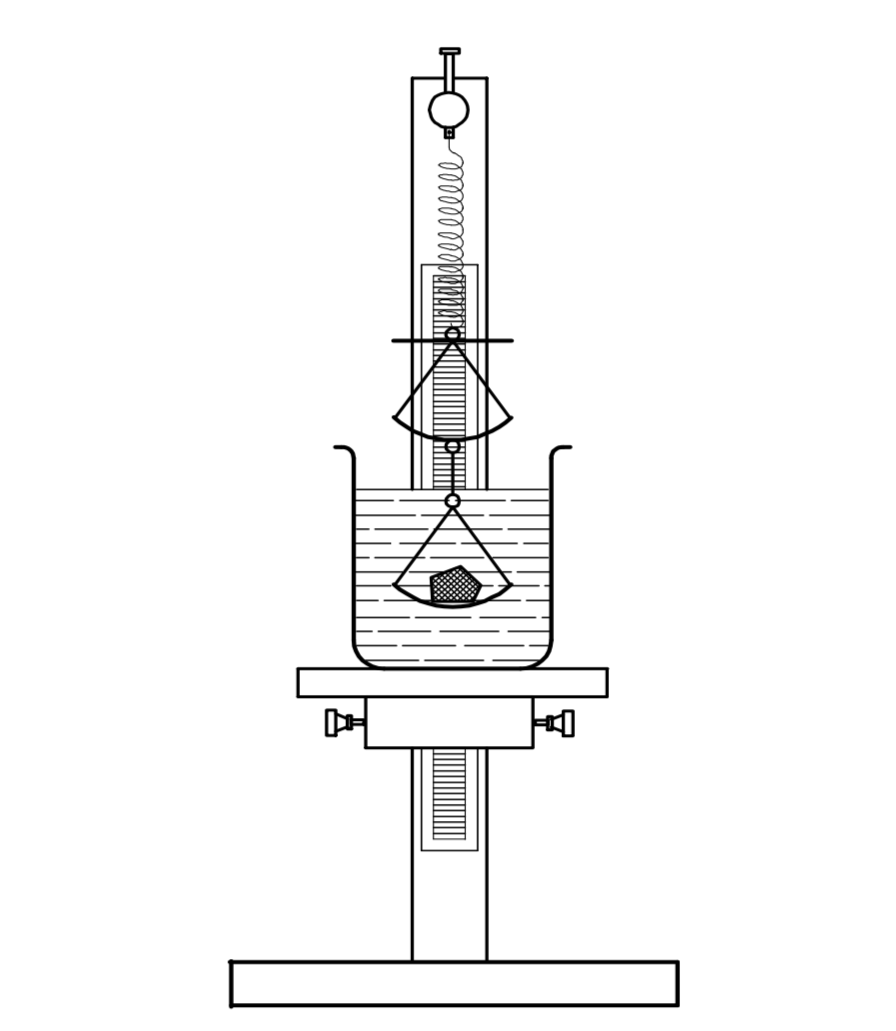
\includegraphics[width=0.6\textwidth]{JollySketch}}
   \renewcommand\thefigure{B1}
\caption[Jollysche Federwaage]{Jollysche Federwaage \cite{Anleitung}}
\label{JS1}

\end{minipage}
\end{figure}

\subsection{Durchführung}

Anfangs wurde die Kugel mit der oberen Waagschale gewogen, und dann mit der im Wasser getunkten Waagschale. Zunächst wurde der verschiebbare Tisch auf dem sich der Becher befindet Verstellt und den Aufhängepunkt der Feder so eingestellt, dass die Waagschale wieder gleich tief in dem Wasser ist. Dann wird noch mal gewogen und das ganze für fünf verschiedene Positionen wiederholt. 

Dann wird das Wasser mit der unbekannten Flüssigkeit ersetzt und das Verfahren wurde nochmals fünf mal wiederholt.

\subsection{Auswertung}

Zur ersten Aufgabe:\\
Die Messungen wurden mit einer Metallkugel durchgef\"uhrt mit einem Durch\-messer von $d=(1.2\pm0.03)$cm und einer Masse von $m=(7.03\pm0.005)$g. Mit der Formel f\"ur das Volumen, $V=\frac{\pi}{6}d^3$, und f\"ur die Dichte, $\rho=\frac{m}{V}$, ergibt sich ein Wert von $(7810\pm550)\mathrm{\nicefrac{\textrm{kg}}{m^3}}$. Hierbei wurde der Fehler \"uber die Potenz\-formel des Gau\ss 'schen Fehlerfortpflanzungsgesetzes ($\delta V=\frac{\Delta V}{V},\ \delta V=3\delta d$) bei Vernachl\"assigung des Fehlers der Masse bestimmt.\\

\begin{table}[h]
\caption{Messwerte Kugel}
$$
 \begin{array}{ll}
 	 \textrm{In Wasser}: \\ \textrm{werte in mm} \\ \textrm{Fehler: $\pm 0.1$mm}
 \end{array}
\rowcolors{2}{gray!10}{white}
\noindent%
\begin{tabular}{|l r| ccccc|}
\hline
Messung && 1 & 2 & 3 & 4 & 5\\
\hline
Ruhelage & $x_0$ & 441 & 479 & 473 & 463 & 468\\
Nicht eingetaucht & $x_1$ & 414 & 453 & 447 & 436 & 440\\
Eingetaucht & $x_2$ & 417 & 456 & 450 & 439 & 443\\
\hline
\end{tabular} \phantom{\begin{array}{ll}
 	 \textrm{In Wasser}: \\ \textrm{werte in mm} \\ \textrm{Fehler: $\pm 0.1$mm}
 \end{array}
}$$
\end{table}

F\"ur das Dichteverh\"altniss gilt:\\

\begin{equation}
\frac{\rho}{\rho_{Fl}} = \frac{F_G}{F_G - F_{G'}}\label{eq2}
\end{equation}

\begin{equation}
F = -k(x-x_0)\mathrm{,}\label{eq3}
\end{equation}

wobei die Gr\"o\ss en in (\ref{eq2})
\begin{itemize}
  \item $\rho$ und $\rho_{Fl}$ jeweils die Dichten von dem K\"orper und der Fl\"ussigkeit.
  \item $F_G$ die Gewichtskraft des K\"orpers in Luft.
  \item $F_{G'}$ die Gewichtskraft des K\"orpers in einer Fl\"ussigkeit.
\end{itemize}

und in (\ref{eq3})
\begin{itemize}
  \item $F$ die Federkraft
  \item $k$ die Federkonstante
  \item $x_0$ die Ruhelage der Waage
  \item $x$ die Auslenkung der Waage sind.
\end{itemize}

Daraus ergibt sich f\"ur die Dichte mit den Auslenkungen $x_1$ Objekt in Luft und $x_2$ Objekt in Fl\"ussigkeit:
\begin{equation}
\rho=\rho_{Fl}\frac{x_1-x_0}{x_1-x_2}.\label{eq1}
\end{equation}
F\"ur unsere Messwerte aus Tabelle 1 erhalten wir

\begin{table}[h]
\caption{Dichte Kugel}
$$\begin{tabular}{|c|c|c|c|c|c|}
\hline
\textrm{Messung} & 1 & 2 & 3 & 4 & 5\\
\hline
$\textrm{Dichte }\rho\left[\nicefrac{\textrm{kg}}{\textrm{m}^3}\right]$ & $8982\pm4260$ & $8649\pm4104$ & $8649\pm4104$ & $8982\pm4260$ & $9314\pm4416$\\
\hline
\end{tabular} $$
\end{table}

Der Mittelwert unserer Messung betr\"agt also $\rho=(8900\pm1800)\mathrm{\nicefrac{\textrm{kg}}{m^3}}$. Diese Rechnungen wurden mit dem \textit{uncertainties} Paket in Python durchgef\"uhrt. \refpy{1}. \cite{Uncertainties}

%\begin{figure}[p]
%\centering
%\fbox{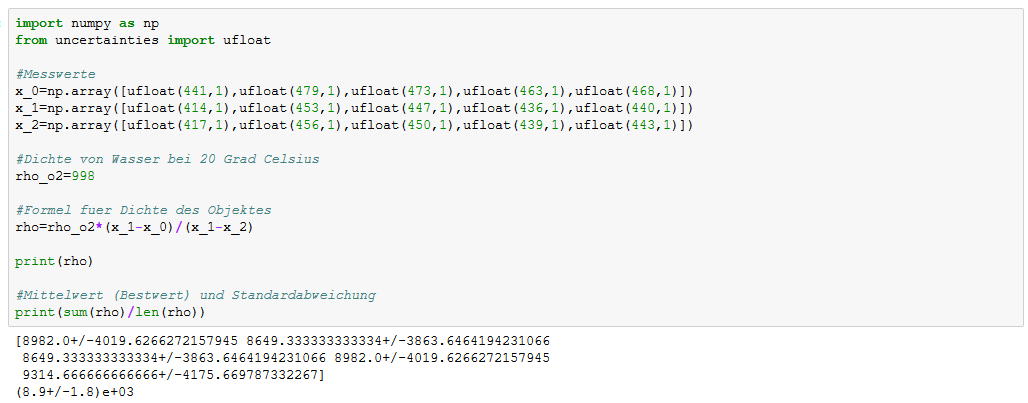
\includegraphics[width=1\textwidth]{Rechnung_1.PNG}}
%   \renewcommand\thefigure{A1}
%\caption{Rechnungen mit Python und $uncertainties$ Paket.}
%\label{ab1}
%\end{figure}

%\begin{figure}[p]
%\centering
%\includegraphics[width=0.6\textwidth]{Rechnung_3.PNG}
%   \renewcommand\thefigure{A3}
%\caption{Rechnungen mit Python und $uncertainties$ Paket.}
%\label{ab5}
%\end{figure}


Der Fehler der Messung mit der Jollyschen Waage ist aufgrund des gro\ss en Dichteunterschieds zwischen dem Metall und der Fl\"ussigkeit so gro\ss. Dadurch ist die Auftriebskraft im Vergleich zur Gewichtskraft der Kugel klein und man erh\"alt im Nenner von (\ref{eq1}) die Differenz zweier nahezu gleichen Messwerte, deren Fehler dann gro\ss\ ist.\\

Zur zweiten Aufgabe:\\
Die Rechnungen wurden mit den Messwerten aus dem ersten Aufgabenteil durchgef\"uhrt und es wurde die gleiche Apparatur verwendet. Als Wert f\"ur die Dichte des K\"orpers wurde der Mittelwert auf dem ersten Aufgabenteil genutzt. Die Formel (\ref{eq1}) wurde zu
\begin{equation}
\rho_{Fl}=\rho\frac{x_1-x_2}{x_1-x_0}\label{eq4}
\end{equation}
umgestellt.

F\"ur die unbekannte Fl\"ussigkeit wurde gemessen:

\begin{table}[h]
\caption{Messwerte Flüssigkeit}
$$
 \begin{array}{ll}
 	 \textrm{In Fl\"ussigkeit}: \\ \textrm{werte in mm} \\ \textrm{Fehler: $\pm 0.1$mm}
 \end{array}
\rowcolors{2}{gray!10}{white}
\noindent%
\begin{tabular}{|l r| cccc|}
\hline
Messung && 1 & 2 & 3 & 4\\
\hline
Ruhelage &$x_0$ & 449 & 466 & 440 & 482\\
Nicht eingetaucht &$x_1$ & 424 & 438 & 414 & 455\\
Eingetaucht &$x_2$ & 427 & 441 & 417 & 458\\
\hline
\end{tabular} \phantom{\begin{array}{ll}
 	 \textrm{In Fl\"ussigkeit}: \\ \textrm{werte in mm} \\ \textrm{Fehler: $\pm 0.1$mm}
 \end{array}
}$$
\end{table}

Mit (\ref{eq4}) ergibt sich dann:

\begin{table}[h]
\caption{Dichte Flüssigkeit}
$$\begin{tabular}{|c|c|c|c|c|c|}
\hline
\textrm{Messung} & 1 & 2 & 3 & 4\\
\hline
$\textrm{Dichte }\rho\left[\nicefrac{\textrm{kg}}{\textrm{m}^3}\right]$ & $1068\pm523$ & $953\pm469$ & $1026\pm504$ & $989\pm486$\\
\hline
\end{tabular} $$
\end{table}

Hier ist der Mittelwert dann $\rho_{Fl}=(1010\pm300)\mathrm{\nicefrac{\textrm{kg}}{m^3}}$. Die Rechnungen wurden hier wieder mit dem $uncertainties$ Paket in Python durchgef\"uhrt. \refpy{2}. 

%\begin{figure}[p]
%\centering
%\fbox{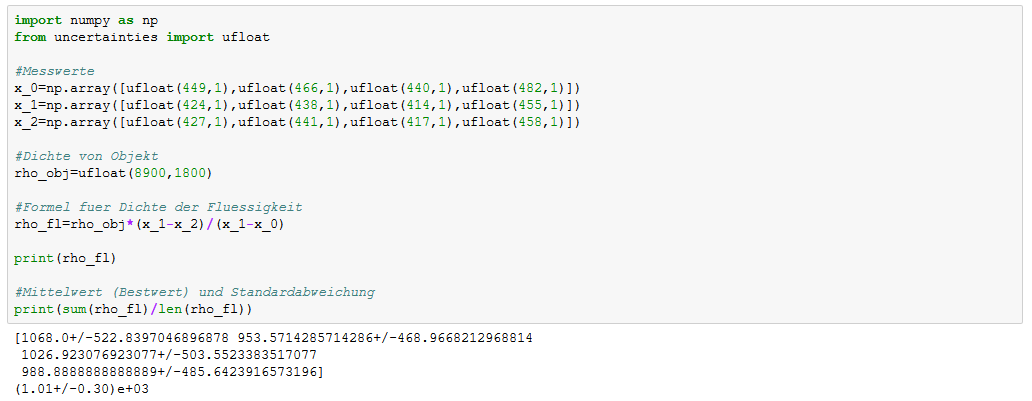
\includegraphics[width=0.8\textwidth]{Rechnung_2.PNG}}
%   \renewcommand\thefigure{A2}
%\caption{Rechnungen mit Python und $uncertainties$ Paket.}
%\label{ab2}
%\end{figure}

\subsubsection{Unsicherheitsvergleich mit Streuung}

Aus den 5 bzw. 4 Einzelwerten der beiden Messungen ergeben sich folgende Streuungen:\\

$$s_\rho=279\, \mathrm{\nicefrac{\textrm{kg}}{m^3}},\quad s_{\rho_{Fl}}=49.1\, \mathrm{\nicefrac{\textrm{kg}}{m^3}}$$

Diese Werte sind erheblich kleiner als erwartet. Der Grund daf\"ur k\"onnte bei einer zu groben Absch\"atzung der Messungenauigkeit oder aufgrund der geringen Anzahl an Einzelmessungen (5 bzw. 4) liegen.\\

Geht man von einer halb so gro\ss en Messungenauigkeit aus, so erh\"alt man Fehlerabsch\"atzungen von etwa 2000 $\mathrm{\nicefrac{\textrm{kg}}{m^3}}$, was immer noch nicht konsistent mit der Absch\"atzung mittels $s_\rho$ ist. Daher m\"ussen wir davon ausgehen, dass die kleinen Werte von $s_\rho\textrm{ und}\ s_{\rho_{Fl}}$ durch die geringe Anzahl an Einzelmessungen zustande gekommen sind.\\

Aus den Unsicherheiten der Einzelmessungen ergeben sich Standardabweichungen des Mittelwerts von:\\
\[
s_{\overline{\rho}}=(3987\pm125)\nicefrac{\textrm{kg}}{m^3},\quad
s_{\overline{\rho_{Fl}}}=(505\pm25)\nicefrac{\textrm{kg}}{m^3}
\]

Bei der Messreihe mit der unbekannten Fl\"ussigkeit gibt es einen systematischen Fehler aufgrund der verwendeten gemessenen Dichte des K\"orpers, die unter umst\"anden zu gro\ss\ oder zu klein gesch\"atzt wurde und als Referenz dient.
\pagebreak

\section{Teil B - Oberfl\"achenspannung}

\subsection{Aufbau}

\begin{figure}[h]
\begin{minipage}{.6\textwidth}
Für diesen Versuchsteil wird eine Torsionswaage verwendet. Zusätzlich werden zwei gleiche Drahtbügel verwendet. Benötigt wird noch Ethanol, um die Drahtbügel von Fettspuren zu reinigen. Ein kleinen Becher der zuerst mit Wasser und später mit Ethanol gefüllt wird. An den enden der Waage befindet sich jeweils ein Häkchen wo die Drahtbügel angehängt werden. 
\end{minipage}%
\begin{minipage}{.4\textwidth}
\centering
\fbox{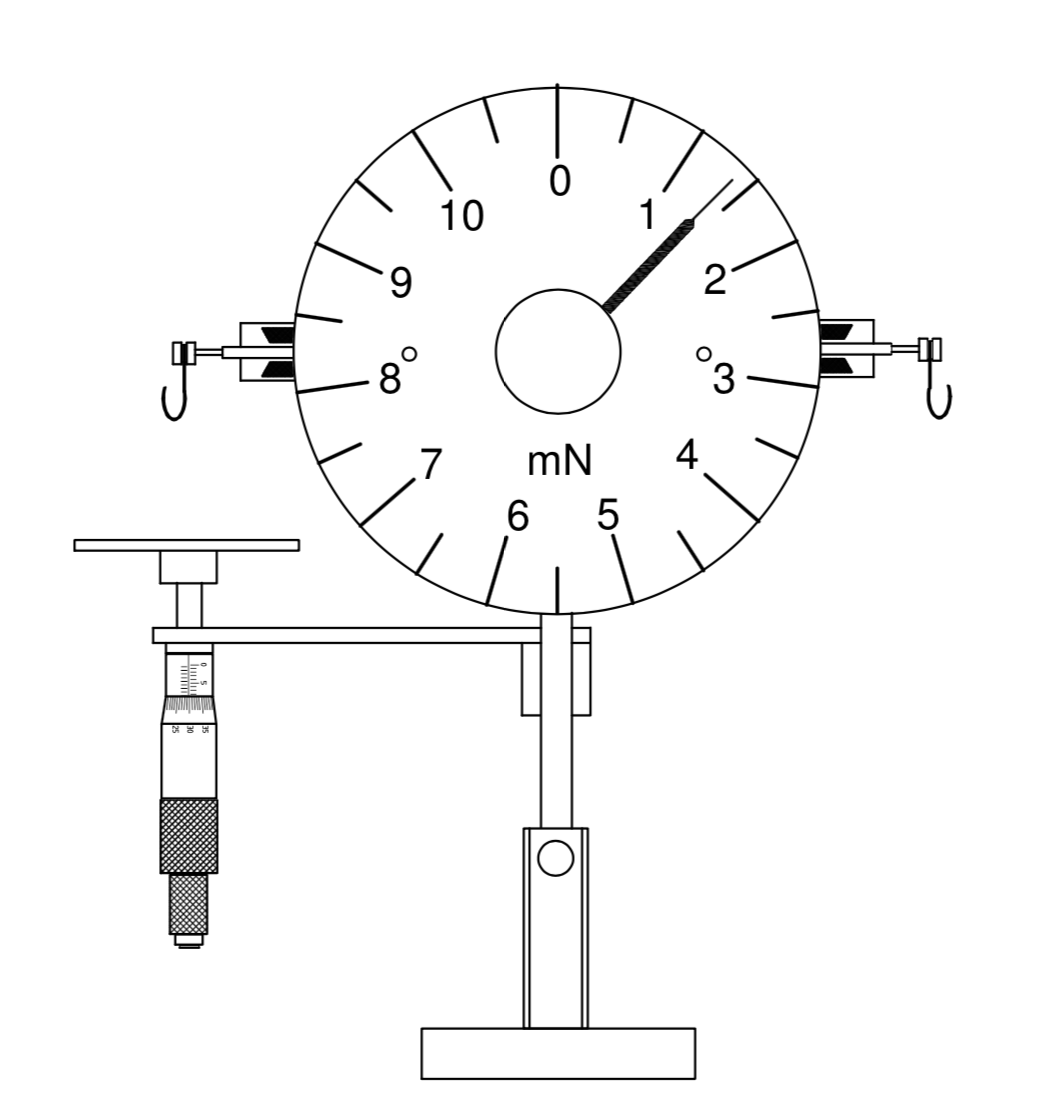
\includegraphics[width=0.7\textwidth]{NewtSketch.PNG}}
   \renewcommand\thefigure{B2}
\caption[Torsionswaage]{Torsionswaage \cite{Anleitung}}
\label{NS1}
\end{minipage}
\end{figure}

\subsection{Durchführung}

Erst wurden die Drahtbügel mit dem Ethanol gewischt, dann gewogen. Die Drahtbügel werden an die Häkchen gehängt und der Wasserbecher wird auf den Messtisch unter dem linken Drahtbügel gestellt. Als nächstes wurde die Waage kalibriert und die Auftriebskraft des Wassers ausgeglichen. Hierzu wird zuerst die Kraftwaage auf null gestellt, um den Gewicht unterschied auszugleichen. Zunächst wird der Drahtbügel in das Wasser getunkt und der Messtisch so eingestellt, dass die an dem Drahtbügel gebildete Lamelle gerade reißt. Die Auftriebskraft wird dann ausgeglichen durch abwechselndes drehen der beiden Knöpfe an der Kraftwaage. Danach wurde der Drahtbügel wieder in das Wasser getunkt und die Lamelle erneut gebildet. Dann wird die Kraft gemessen die an dem Punkt auftritt genau vor die Lamelle reißt. 

\subsection{Auswertung}
Die Oberfl\"achenspannung von Wasser und Ethanol wurde mit der Abrei\ss methode gemessen. F\"ur diese gilt:
\begin{equation}
\sigma=\frac{F_{s_{max}}}{2l}\label{eqo}
\end{equation}
% (\ref{ab3}) und (\ref{ab4})
Die L\"ange $l$ des Drahts betr\"agt $2.63\pm0.03$ cm. Die Messwerte befinden sichf\"ur Wasser und Ethanol befinden sich im Anhang. Deren Graphische Darstellungen in den Graphiken sind auch im Anhang. Die Sigmoidfunktion 
\begin{equation}
d\times\frac{1}{1+\exp(-c\times(x-a))}+b
\end{equation} 
wurde mit der curve\_fit Funktion von dem SciPy Paket in Python an die Messpunkte angepasst. Aus den Graphiken lesen wir folgende Werte f\"ur $F_{s_{max}}$ ab:

\begin{table}[h]
\caption{Kräfte bei Wasser}
$$\begin{tabular}{|c|c|c|}
\hline
\textrm{Messung} & 1 & 2\\
\hline
$\textrm{Kraft }F_{s_{max}}\ \mathrm{[mN]}$ & $5.16\pm1.03$ & $4.75\pm0.95$\\
\hline
\end{tabular} $$\label{tabfmw}
\end{table}

\begin{table}[h]
\caption{Kräfte bei Ethanol}
$$\begin{tabular}{|c|c|c|c|}
\hline
\textrm{Messung }$$ & 1 & 2 & 3\\
\hline
$\textrm{Kraft }F_{s_{max}}\ \mathrm{[mN]}$ & $1.27\pm0.25$ & $1.42\pm0.28$ & $1.38\pm0.28$\\
\hline
\end{tabular} $$\label{tabfme}
\end{table}
\FloatBarrier

Die Fehler wurden durch Streuung der Messpunkte um die angepassten Kurven abgesch\"atzt.

Mit der Formel (\ref{eqo}) ergibt sich f\"ur die Oberfl\"achenspannung 

\begin{table}[h]
\caption{Oberflächenspannung bei Wasser}
$$\begin{tabular}{|c|c|c|c|}
\hline
\textrm{Messung} & 1 & 2 & Mittelwert\\
\hline
$\textrm{Oberfl\"achenspannung [\nicefrac{mN}{cm}}]$ & $0.98\pm0.20$ & $0.90\pm0.18$ & $0.94\pm0.13$\\
\hline
\end{tabular} $$\label{tabow}
\end{table}

\begin{table}[h]
\caption{Oberflächenspannung bei Ethanol}
$$\begin{tabular}{|c|c|c|c|c|}
\hline
\textrm{Messung }$$ & 1 & 2 & 3 & Mittelwert\\
\hline
$\textrm{Oberfl\"achenspannung [\nicefrac{mN}{cm}}]$ & $0.24\pm0.05$ & $0.27\pm0.05$ & $0.26\pm0.05$ & $0.26\pm0.03$\\
\hline
\end{tabular} $$\label{taome}
\end{table}

\vfill

\begin{thebibliography}{9}
\bibitem{Uncertainties}''Correlations between variables are automatically handled, which sets this module apart from many existing error propagation codes.'' - https://pythonhosted.org/uncertainties/
\bibitem{Wasser} \url{https://en.wikipedia.org/wiki/Surface-tension_values#cite_note-one-2} (\today)
\bibitem{Ethenol} \url{https://en.wikipedia.org/wiki/Surface_tension} (\today)
\bibitem{Anleitung} Physikalisches Institut der Albert-Ludwigs-Universität Freiburg (Hrsg.) (08/2018): Versuchsanleitungen zum Physiklabor für Anfänger*innen, Teil 1, Ferienpraktikum im Sommersemester 2018.
\end{thebibliography}

\pagebreak

\section{Anhang: Tabellen und Diagramme}

\begin{table}[h]
\centering
\caption{Messwerte für Wasser (Teil B)} \vspace{11pt}
$\begin{array}{l}
\textrm{Unsicherheiten:}\\
\textrm{Höhe: } \pm 0.03 \textrm{mm}\\
\textrm{Kraft: } \pm 0.02 \textrm{mN}
\end{array}$
\begin{tabular}{ccc}
\toprule
\textrm{H\"ohe}/\textrm{mm}& \textrm{Kraft}/\textrm{mN} & \textrm{Kraft}/\textrm{mN} \\
\midrule 
2 & 0.26 & 0.23\\
\hline
4 & 0.33 & 0.25\\
\hline 
5 & & 0.3\\
\hline 
6 & 1.25 & 0.83\\
\hline 
8 & 3.9 & 0.83\\ 
\hline
9 & 4.75 & 4.6\\ 
\hline
10 & 4.7 &\\ 
\bottomrule
\end{tabular}
\phantom{$\begin{array}{l}
\textrm{Unsicherheiten:}\\
\textrm{Höhe: } \pm 0.03 \textrm{mm}\\
\textrm{Kraft: } \pm 0.02 \textrm{mN}
\end{array}$}
\label{tabmw}
\end{table}

\begin{table}[h]
\caption{Messwerte für Ethanol (Teil B)} \vspace{11pt}
\centering
$\begin{array}{l}
\textrm{Unsicherheiten:}\\
\textrm{Höhe: } \pm 0.03 \textrm{mm}\\
\textrm{Kraft: } \pm 0.02 \textrm{mN}
\end{array}$
\begin{tabular}{cccc}
\toprule
\textrm{H\"ohe}/\textrm{mm}& \textrm{Kraft}/\textrm{mN} & \textrm{Kraft}/\textrm{mN} & \textrm{Kraft}/\textrm{mN} \\
\midrule 
0 & -0.35 & -0.35 & \\
\hline
1 & -0.2 & & \\
\hline 
3.5 & & & 0\\
\hline 
3.75 & 0 & 0 & \\
\hline 
4 & & & 0.15\\ 
\hline
4.5 & & & 4.6\\ 
\hline
5 & 0.67 & 0.85 & 1.1\\ 
\hline
5.5 & & 1.1 & 1.25\\ 
\hline
6 & & 1.3 & 1.4\\ 
\hline 
6.2 & & & 1.43\\ 
\hline
6.4 & & & 1.4\\ 
\hline
6.5 & & 1.35 & \\ 
\hline
6.6 & & & 1.3\\ 
\hline
7 & 1.25 & & \\ 
\hline
8 & 1.25 & &\\
\bottomrule 
\end{tabular}
\phantom{$\begin{array}{l}
\textrm{Unsicherheiten:}\\
\textrm{Höhe: } \pm 0.03 \textrm{mm}\\
\textrm{Kraft: } \pm 0.02 \textrm{mN}
\end{array}$}
\label{tabme}
\end{table}

\begin{figure}[p]
\centering
\fbox{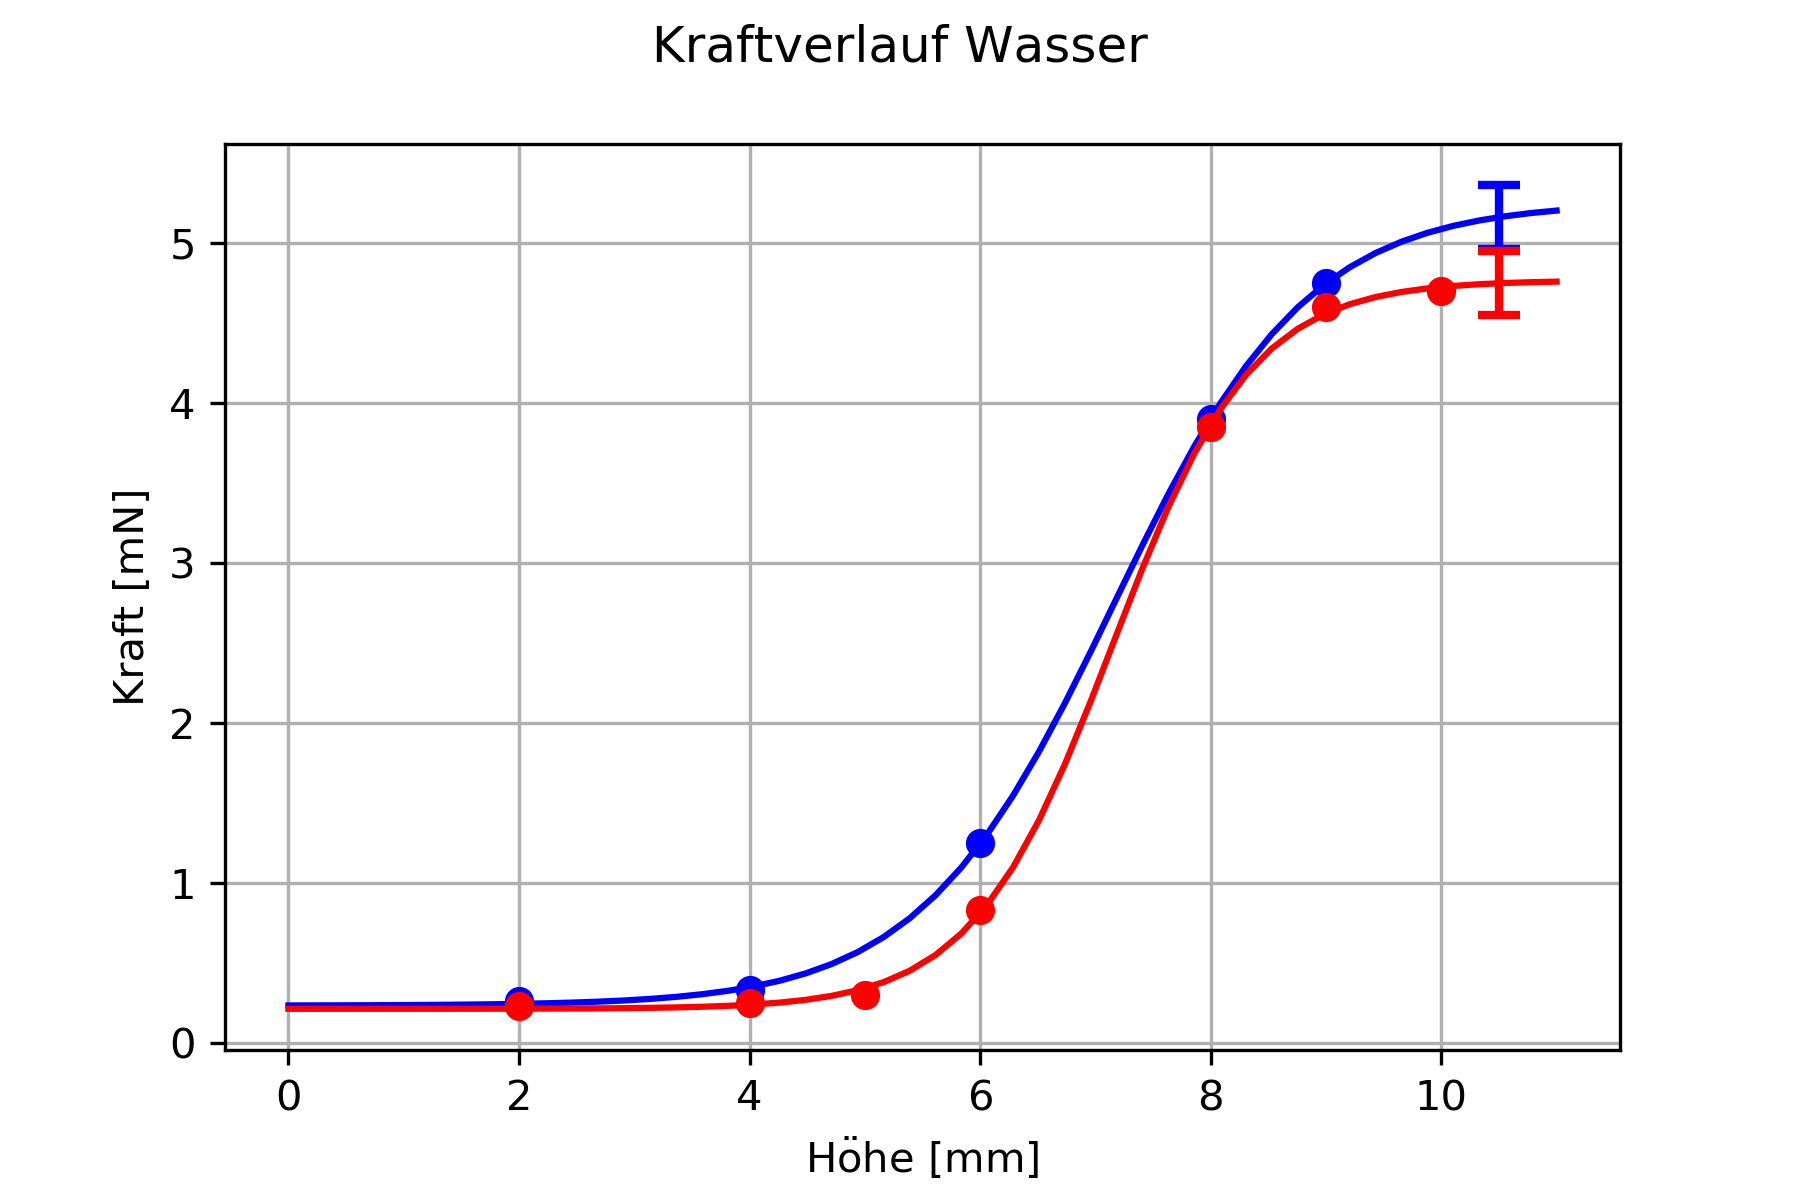
\includegraphics[width=0.8\textwidth]{Graph_1.png}}
\renewcommand\thefigure{B3}
\caption[Kraft/Höhe Diagramm Wasser]{Verlauf der Kraft $F$ als Funktion der Position $x$ beim Herausziehen des B\"ugels aus der Fl\"ussigkeit.}
\label{ab3}
\end{figure}

\begin{figure}[p]
\centering
\fbox{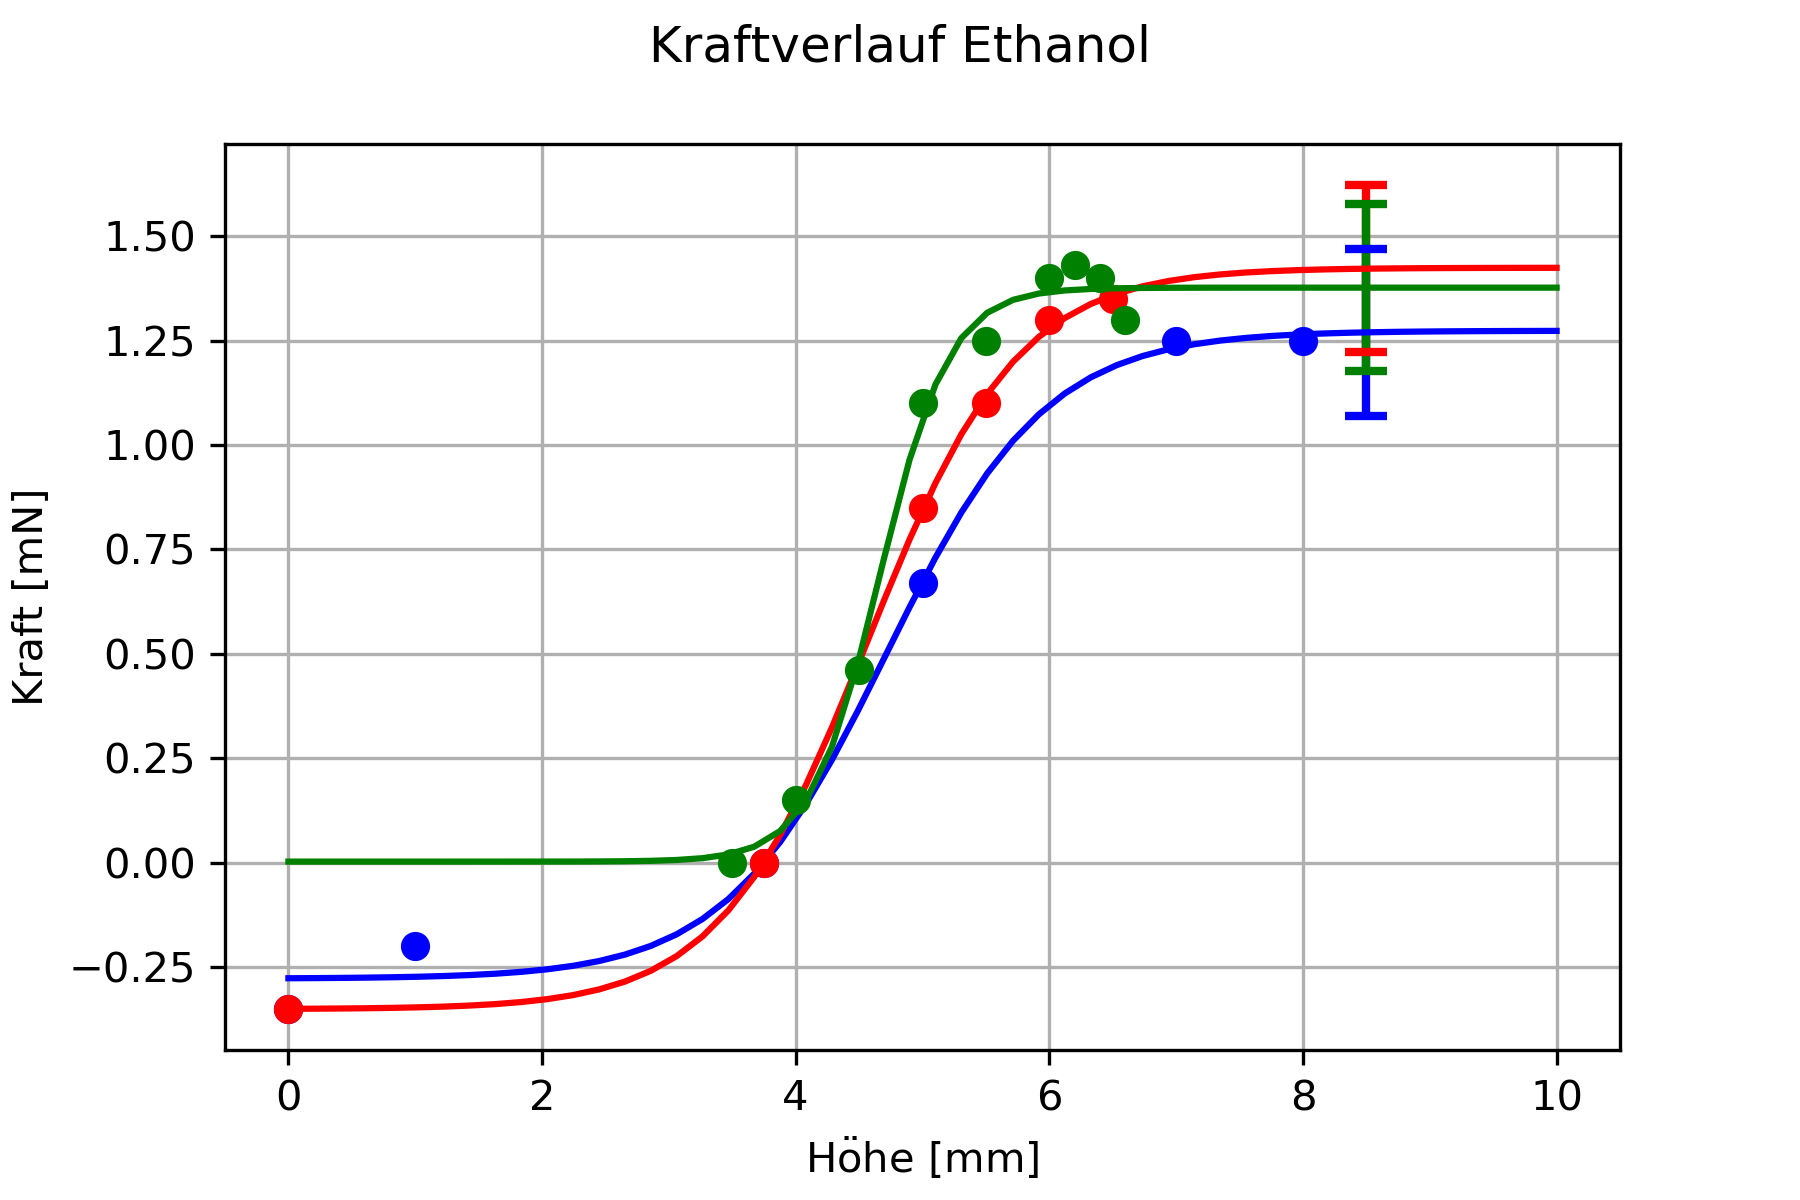
\includegraphics[width=0.8\textwidth]{Graph_2.png}}
\renewcommand\thefigure{B4}
\caption[Kraft/Höhe Diagramm Ethanol]{Verlauf der Kraft $F$ als Funktion der Position $x$ beim Herausziehen des B\"ugels aus der Fl\"ussigkeit.}
\label{ab4}
\end{figure}

\end{document}